
\textcolor{blue}{
The details of the language models developed for the Wakirike language is discussed in this chapter.  The language models developed draw  upon the premise that the grammar of a language is expressed in the character sequence pattern ultimately rendered in word sequences.  The two models developed in this chapter follow RNN implementations discussed in chapter \ref{ch3RNN}. }

\section{Data Preparation}
\startblue
A published version of the Wakirike New Testament Bible was obtained and used as the data source for RNN training of the language model.  There was no readily available soft or online copy of the Wakirike new testament bible. As such, the Wakirike New Testament Bible text corpus text was entered into the ASR system from the physical copy using a text editor to form a text corpus.  The complete corpus had a word count of 668,522 words and a character count of 6,539,176 characters. Following the k-fold cross validation process \citep{geron2019hands}, the data set was then divided into 11 parts. Two parts dedicated for testing and validation and the remaining nine parts were used for training. As the validation set is not seen during training it can be used to keep track of how well the training is going and that it is not over-fitting the data by simply memorising it.

Preprocessing of the text corpus involved selecting a set of characters as the input feature set and removing all other characters not found in the input feature set.  The Unicode representations of the character set consisted of letters and punctuation marks.  These are one-hot encoded and batched for sequential input.  Neural network parameters which are not automatically determined through back propagation are called hyper-parameters.  These are usually experimentally determined and manually set while configuring the network.  A hyper-parameter for the language model RNN is the input sequence length.  For the language model built a 30 characters-long sequence length is chosen.  This  length is an average phrase sequence.  In these phrases, long-term character dependencies of words can be captured. At the same time, keeping the sequence length at this value, and not longer, will pose less of a burden on the computer system resources during parameter computations.  

Another hyper-parameter for training used was the batch size.  The batch size parameter determined how many 30-character sequences will be trained in parallel in order to speed up the training process.  Increasing the batch size also meant an increase in the size of the matrix multiplications being performed and therefore, the computing power system resource being demanded by the language model.  By experimenting with various batch sizes it was determined a batch size of 200 was suitable for training the language model with respect to the other training parameters.

\section{General Considerations for Sequence-to-sequence modelling}\label{sec_c6_seqdesign}
The systems built in this work is centred around \acrfull{dnns}.  A \acrshort{dnn}, is a function approximator of some function $f\ast$. The sequence models developed in this work are based on \acrshort{dnns}.  The models can therefore be viewed simply as mappings from inputs to outputs.  While the inputs and outputs may vary from one system to another along with that of the design of the \acrshort{dnn}s implemented, these models share common features that aim towards the common goal of function approximation.  

In Chapter \ref{ch1_intro}, it is mentioned that the systems developed in this work fall under the class of problems known as pattern recognition tasks, whether it be recognition of speech patterns or that of language patterns for language models.  They are therefore also grouped into the branch of machine learning algorithms known as classifiers.  \cite{Goodfellow-et-al-2016} formalises a classifier as the function $y=f∗(x)$, which based on a set of learnable parameters, $\theta$, maps an input $x$ to a category $y$. Therefore defines
\begin{equation}\mathbf{y}=f(\mathbf{x;\theta})  \end{equation}\label{eq_c6_classifier}

The General criteria considered in this section is a continuation of all the design considerations for sequence models defined in Section \ref{sec_postalign} and Section \ref{sec_341_rnnproc}.  These defined criteria represent the features of the network that vary from one sequence design to another and ultimately have influence on the learnable parameters, $\mathbf{\theta}$ of our \acrshort{dnn}-based \acrshort{rnn}-sequence model. The following paragraphs therefore discuss these hyper parameters and their selections for the three sequence models involved in empirical analysis in this study.

\subsection{Selection of Sequence Model}\label{sec_c6_seqsel}
In this Section \ref{sec_postalign}, we establish different sequence models types (see Figure \ref{fig_c3_seq2seq}) and the rationale for only using \acrshort{mimo} for our systems as being due to the fact that for speech and language  which are modeled in this work, we have the inputs and the outputs as time series data. Therefore our sequential models can indeed be modelled as \acrshort{mimo} sequences and would only need to either be modelled as synchronous or asynchronous \acrshort{mimo}.

For the design of the character-based language sequence model, the idea is that since the language rules are expressed in the character sequence, then, for each input in the training data the most accurate next character based on all the previous characters leading to the current would be the next found in the training sequence.  Therefore, there is only one corresponding output and vice versa, hence, we use a synchronous \acrshort{mimo} relationship to model the language model.

In this work, there are two speech models developed for low resource end-to-end \acrshort{asr}.  The first is based on the synchronous \acrshort{mimo} design and the second is based on the asynchronous details of these designs are given in Sections \ref{sec_c7_birnn} to \ref{sec_c7_baseline}. For both of these regardless, the \acrshort{ctc} algorithm ensures the asynchronous \acrshort{mimo} relationships between inputs and outputs are restored.

\subsection{Selection of RNN-architectures for sequence modelling}
In the previous section (\ref{sec_c6_seqsel}) and in Section \ref{sec_postalign}, five \acrshort{rnn}/\acrshort{dnn} sequence-to-sequence models were defined as 
\acrfull{siso}
\acrfull{miso}
\acrfull{simo}
Synchronous \acrfull{mimo}
Asynchronous \acrfull{mimo}

Note that number 1 above can only apply to a regular \acrshort{dnn}, while numbers 2 to 5  apply to \acrshort{rnn}s.  Apart from the super-structures, the second sequence-to-sequence design criteria considers the sub-structures that comprise these super structures at the cell level.  There are five of \acrshort{rnn} sub architecture considered in this work
Regular \acrshort{dnn}s
\acrfull{lstm}
\acrfull{gru}
\acrlong{birnn}
\acrlong{blstm}

Chapter \ref{ch5_DNN} presented an in-depth look at the above \acrshort{rnn} sub-structures.  For the \acrshort{rnn}-\acrshort{lm} developed in this Chapter, the sub-structure selected was the \acrshort{gru}. Similarly, the \acrshort{bilstm} is used for first speech model experiments. Details of the designs and selection criteria are given in this Chapter and Chapter \ref{ch6_speech}.  Note however, that as the name implies, the \acrfull{blstm} is a \acrshort{birnn} where the regular \acrshort{rnn}s are replaced by \acrshort{lstm}s.  Furthermore, the results in this Chapter show that there was no need to use the heavier duty \acrshort{lstm}s or \acrshort{birnn}s for the language model development  as the deep-\acrshort{gru}s proved to be quite sufficient. Speech models however, required a more robust substructure where \acrshort{blstm} have been shown to perform better \citep{kim2017joint}.

\subsection{Neural Network geometry}
Neural network geometry refers to the number of layers and the number of neurons per layer. This will give the total degrees of freedom of the neural network.  Increasing the number of neurons per layer causes the neural network to extend the dimensions for discrimination.  However, increasing the number of layers enables better generalisation of the dimensional data.  These parameters have been selected empirically based on pilot experiments and experiments on neural networks for similar research. Generally for neural networks involving \acrshort{rnn}s good practice should have the number of layers start from 2-layers and the number of neurons per layer from 64.  Experiments for this research typically had 3-5 layers with the number of neurons being between 128 and 2048.

\subsection{Network Saturation Parameters}
The succeeding paragraphs discuss parameters that are selected to either ensure that the network trains in a stable manner that saturates or that tries to assist the network to train faster.  Most of these parameters have been selected based on similar research or based on particular types of neural network architectures.
\subsubsection{Weight initialisation} 
These are the values the neuron weights have at the start of training.  If these are  widely ranging values, they tend to make the network unstable.  However, having values that are uniformly distributed around a stable value such as zero ensures that the back propagation adjustments are also changing at a stable rate that favours the gradient descent movement in the data space towards the global optimum. Weight initialisation for models developed in this thesis followed this Gaussian initialisation and that of common stable weight initialisation models such as Xavier initialisation \citep{kumar2017weight} or Glorot initialisation \citep{glorot2010understanding} .
\subsubsection{Non-Linear function selection}
In Chapter \ref{ch3RNN}, the following nonlinear functions sigmoid, tanh and \acrshort{relu} were introduced.  These functions enable neural networks to navigate nonlinear space as function approximators.  Out of these three nonlinear functions, only \acrshort{relu}s \citep{he2015delving} are immune to the “vanishing gradient problem”.  As identified in \cite{glorot2010understanding}, the vanishing gradient problem seen in very deep neural networks where gradients get smaller while back propagating through the network and quickly become zero and stopping the network from saturating at that point. Due to the hidden layers of the \acrshort{rnn}, they constitute very deep networks and therefore susceptible to the “vanishing” gradient problem.  The three models main models developed in this work use clipped \acrshort{relu}s for activation.
\subsubsection{Number of epochs}
An epoch is an event that occurs when the neural network has processed all the training data available.  Neural networks iteratively get trained until the network saturates or has reached an optimal state where the performance cannot improve further.  Usually, it takes several epochs for the network to get to a global optimum assuming all other parameters are configured optimally.  In the models developed in this thesis, the number of epochs were selected empirically from pilot experiments.  In some of the experiments performed, epochs were selected based on the Research objectives not to train for more than a few hours for the language models or a few days for speech models.
\subsubsection{Learning rate}
Learning rate has been introduced in Chapter \ref{ch3RNN}. The rule of thumb for \acrshort{dnn}s is the larger the network the lower the learning rate should be.  Learning rates applied to sequence models developed in this work based on geometries used ranged from 0.0001 to 0.0005.
6.2.4.5 Cost function selection
We have introduced the root mean square error, negative log likelihood and the \acrshort{ctc} loss cost functions in Chapter \ref{ch3RNN}.  This work made use of the negative log likelihood for the language model and the \acrshort{ctc} for the speech models. By way of comparison the AutoSegCriterion \citep{collobert2016wav2letter} is reviewed.
\subsubsection{Optimiser}
Gradient descent algorithm has been introduced in Chapter \ref{ch3RNN}.  Different algorithms that improve upon the Gradient descent algorithm, such as ensuring a global minima is determined, are explored in work.  The adadelta and adam optimizer are examples of such used in this thesis.

\subsection{Regularisation measure}
Rather than adjusting neural network geometry in order to find an optimal geometry that neither over fits or under fits the data, a common way to avoid over fitting the data is by a method known as dropout \citep{srivastava2014dropout}.  Dropout was the regularisation strategy employed by this research.  Dropout will therefore determine which neurons will refrain from emitting its output at each layer. Using similar research, dropout values were 20\% for the language model and 10\% for \acrshort{birnn} with attention transducer and 0\% for \acrshort{birnn} only experiments.

\section{GRU RNN Architecture}
The modified LSTM RNN known as the Gated Recurrent Unit (GRU) discussed in Chapter \ref{ch3RNN} is employed for the neural network model built in this Chapter.  In order to optimise network performance while conserving computation resources, GRUs have been shown to give similar performance to regular LSTMs; however, with a lighter system resource footprint \citep{cho2014learning}. 

The architecture of the GRU RNN used to train the Wakirike text corpus had an internal network size of 512 nodes for each layer and was 3 layers deep. In a study by \citep{goodfellow2013multi}, it was shown that increasing the number of nodes in a neural network will lead to over-fitting; however, simultaneously increasing the network depth mitigates this effect.  In other words, in order to expand the degrees of freedom of a neural network and at the same time constrain the network to generalise well on unseen data, it is necessary to increase the number of neurons in both length and depth.  Experiments carried out in this chapter follow this recommendation. Initial experiments had an internal node size of 128 and a single layer deep.  While this showed promise of converging, the error rate was still high, therefore the network was expanded to the final model above.   Externally, the network model is further  sequenced 30 times, representing the input sequence length hyper-parameter and the number of recurrent connections where each connection represents a sequenced time step. 

Another hyper-parameter sensitive to network size is the learning rate.  The learning rate is selected in such a manner that an increase in the network size makes the learning rate more prone to overshooting.  Therefore, increased degrees of freedom in a neural network will require the learning rate to be made smaller so that it does not overshoot the network saturation point.  Small learning rates of between 0.001 and 0.005 were used. Furthermore, the language model neural network was designed to overcome over-fitting using the dropout method \citep{srivastava2014dropout} which has been shown to be effective for regularising deep neural networks.  The hyper-parameter for dropout was kept at 20\% such that only 80\% of neural network activations are propagated from one layer to the next, whereas the remaining 20\% were randomly zeroed out.  Intuitively, dropout works by forcing the remaining active neurons to infer what is missing in the activations that have been dropped and ultimately leads to better generalisations as activations are based on inference than on memory.

\section{Language Model Training Experiments}
Two sets of character-based neural network RNN-based experiments are developed in this chapter.  A third word based statistically modelled language model is also developed based on  \cite{Heafield-estimate} estimates as a baseline model. Character-based perplexity measurements were used to compare the character-based models and a conversion factor based on \citep{hwang2017character} is used to compare character-based models on the word-based counterparts.  Experiments for the RNN language models were majorly performed using tensorflow-MKL, which is a highly parallelised (44-threads for one of the experiments) cpu-based experiments.  The experiment with the largest number of neurons was also performed on cloud-based GPUs (Nvida Tesla T4).  Details of the experiments carried out and resulting perplexity are shown in Table \ref{tab6_1:LMX}.

\begin{table}
  \caption{Language Models comparison}
  \label{tab6_1:LMX}
\begin{tabular}{lrrr}
\toprule
Language Model & Train time & Perplexity & Epochs  \\
\midrule
GRU RNN 3-layer model (CPU training) & ~ 2 days & 30.920 & 75 \\
5-gram with Keysner Soothing and interpolation & 5 minutes & 238.720 & N/A \\
GRU RNN single-layer model (GPU training) & ~ 5 hours & 641491.52 & 120 \\
Plain RNN single-layer model (GPU training) & ~ 9 hours & 27087.893 & 180 \\
GRU RNN 3-layer model (cloud GPU training) & ~ 2 hours & 30.920 & 75 \\
\bottomrule
\end{tabular}
\end{table}

\stopblue


\section{Output Language Model and Language Generation}\label{sec6_4}
\startblue
The 3-layer network experiments were trained on both CPU and GPU configurations. Both were trained for 75 epochs, where an epoch indicates that the model has processed all of the training data.  Recall that the model  is trained until it is saturated.  In other words, the model trains until the prediction accuracy is no longer improving.   This usually will take several epochs.

The loss plots for the three-layer and single layer GRU RNN are shown in Figure \ref{fig_ch7_00losses}.  The three-layer GRU-RNN achieved a prediction accuracy of 65\% on held-out data.  When the created 3-layer GRU character-based RNN language model is seeded with an input character, one can force the network to select from the top-N candidates thus causing the Neural network to generate its own sentences.  In this scenario, the network is said to perform language generation by constructing its own sentences.  The generated language output from the GRU language model was found to be a reflection of the overall context of the training data. 

\begin{figure}
\centering
  % Requires \usepackage{graphicx}
  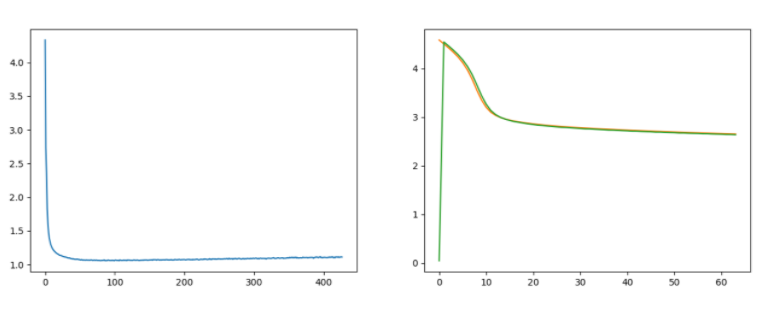
\includegraphics[width=14cm]{thesis/images/losses_slgru}\\
  \caption{Loss curves for a. 3-Layer GRU and b) Single-Layer RNN} \label{fig_ch7_00losses}
\end{figure}

The evaluation of the GRU language model of the Wakirike language was performed using a perplexity measurement metric. The Perplexity metric applies the language model to a test data-set and measures how probable the test data-set is. Perplexity is a relative measure given by the formula:
%
\begin{equation}
PP(W)=P(w_1,w_2\dots w_N)^\frac{1}{N}
\label{ch5_eq1_ppx}
\end{equation}
%
%
\begin{equation}
PP(W)=\sqrt[N]{\prod_{i=1}^N\frac{1}{P(w_i|w_{i-1})}}
\label{ch5_eq2_ppx}
\end{equation}
%
Where $w_1,\dots,w_N$ are the sequence of words. The language model with the lower relative perplexity score is therefore expected to yield better approximation of the data when applied to unseen data generally.

Intuitively, the perplexity metric measures the ability of a language model to predict held-out data.  A character based perplexity metric is possible using  the negative log likelihood of the character sequence.  A character based perplexity metric is possible using  the negative log likelihood of the character sequence.

\begin{equation}
    PP(X)=exp\left\{−\frac{\sum_{t=1}^T\log P(x_t|x_{1:t−1})}{T}\right\}
\label{ch5_eq3_ppx}
\end{equation}

However, our base-line language model is a 5-gram word-based language model.  Therefore, comparing a word based model to a character based model requires a conversion step. In this work, the conversion step involved using the GRU language model generated a corpus which was re-scored by re-estimating with a 5-gram word-based language model

The result of the training of the GRU-Cell Recurrent Neural Network on low-resourced Wakirike Language gave impressive and intelligible results and showed better results when measured with standard n-gram language models. The results showed that it is indeed possible to derive a language model using a GRU-cell RNN on a low resource character sequence corpus for the Wakirike language.
\stopblue

Table \ref{tab6_1:LMX} shows the Results of the Perplexity model of the LSTM Wakirike Language model and an equivalent 5-gram Language model with interpolation and Keysner smoothing \citep{chen1996empirical} for various lengths of the held-out data.
\startblue
\section{Discussion}
The result of the training of the 3-layer-deep GRU-Cell Recurrent Neural Network on low-resourced Wakirike Language had decent results with an accuracy of 65\%.  Even with this accuracy, the model had shown to have learned the vocabulary and was able to construct phrases consistent with the Wakirike language structure.  The single-layer GRU cell however after 120 epochs did not learn the vocabulary and was not able to learn any words.  It can also be seen from the loss curves of the language models that the models reach saturation fairly quickly after about 20 epochs for the 3-layer GRU RNN model and after about 40 epochs for the single-layer RNN.


The results also showed that the 3-layer GRU language model developed a better language model than the 5-gram model in terms of the perplexity metric because the perplexity of the 3-layer GRU RNN model was lower than that of the 5 gram model.  The single layer GRU model being a shallow model with a single-layer did not however learn anything having a  very high perplexity heading towards infinity.  Table \ref{tab6_2:Gen} below demonstrates output generations from the single layer and 3-layer GRU RNN language models based on the sampling procedure described in Section \ref{sec6_4}

\begin{table}
  \caption{Language Models sample generation}
  \label{tab6_2:Gen}
\begin{tabular}{lrrr}
\toprule
a) Original Wakirike Text \\
\midrule
\texttt{mine-o anikanika boro sobie korobo enjelapu so, we duko o piri sa ibiok-}\\
\texttt{wein mi sikima be jinye dukobia bo, ya tamuno worinime sime inibo piri} \\
\texttt{wa tatari duko borosam, a piki mioku bari ani dukoabe na nemikase tomonibo}\\
\midrule
b) GRU RNN 3-layer model (75 epochs) \\
\midrule
 \texttt{ani se mi be chinmgbolu mi ani se chua yee anisiki ini tamuno be bu s-}\\
\texttt{arame, se nwo beme, a kokomaye duko o piriabe, o bi se mi mieari ye mi} \\
\texttt{ori oria koki a kuro mi nyana yee. o bi bara mi o nwose o diebia  ani} \\
 \midrule
c) Plain RNN single-layer model (180 epochs) \\
\midrule
\texttt{min on o o bo oeuemin on o oniaia a bire nami bieee mani o onuo o be} \\
\texttt{bo oe berimini okuma ani mani o o onuaminiana bireme,eanaminianiania b-} \\
\texttt{i bo ono bo onia anaa beremanaa bi nao sike,einama nieiei mi niei ia } \\
\midrule
d) GRU RNN single-layer model (120 epochs) \\
\midrule
\texttt{ia iiiii  o i ii i i iiii  iii i oi oi o oiai  oi ii ii ii  iiiii  i} \\
\texttt{iiii iiiiii  iii iii iii  ii iii  o oi i i o ii iiii  iiii  iiiii i ii} \\
\texttt{i iii i o ii oi oia  oi iiiiii  o i o o o i oi o oi iiiii i iiiii  ii} \\
\bottomrule
\end{tabular}
\end{table}

Table \ref{tab6_2:Gen}(a) to (d) demonstrates how the language generated by various language models resembles the original training data.  The original Wakirike language is given in part (a) then, the other language model generations (following the procedure described in Section \ref{sec6_4}) are shown in order of decreasing similarity.  It can be, therefore, observed that the 3-layer GRU language model had the highest similarity to the original Wakirike language, which has also been evidenced by its low perplexity score.  The other single-layer models having higher perplexity scores showed lesser degrees of similarity to the original Wakirike language.

Finally, it would be in the interest of this research to further consider increasing the number of layers to achieve higher levels of accuracy or consider optimising other parameters which may help the training results, such as the sequence length of the model.  However, this was not done as the time constraint of one day for training the language model was already stretched and we are certain that these hyper-parameters have a direct influence on the size of the model.  This in turn will affect the computing resources required and hence a trade-off of the training time required to saturate the models.

\stopblue

\section{Chapter Summary}
This chapter shows the application of a character-based Gated Recurrent Unit RNN on the low resource language of Wakirike to generate a language model for the Wakirike language.  The data-set and preparation and the details of the network were discussed.  The output of this model was used to hallucinate the Wakirike language which was then scored against word-based perplexity to obtain a metric against the baseline language model.

It can be inferred that the GRU character-model developed has an improved language model and because it is based on a character-model, which is fine-grained when compared to a word model, it is likely to generalise data better when used in practice and is less biased than a word-based model.  This can be observed from the fact that the output corpus produced a larger vocabulary size.
